\chapter{通信网结构}
\section{图论基础}
\subsection{一笔画问题}
\textbf{奇点:}与该条边连接的个数有奇数个\\
\textbf{偶点:}与该条边连接的个数有偶数个\\
一笔画定理:
\begin{itemize}
	\item 中间点一定是偶数点
	\item 最多有两个奇点
	\item 若由偶点组成的连通图,一定可以一笔画,以任意点为起点一以这个点为终点
	\item 只有两个奇点的连通图,一定可以一笔画完;画时以一个奇点为起点,另一个奇点为终点。
\end{itemize}
\subsection{图的基础知识}
\subsubsubsection{基础概念}
\begin{itemize}
	\item 相邻点: vi与vj 互为相邻点( vi 和vj 是一条边的两个端点)
	\item 相邻边:两条边与同一端点相关联,则这两条边为相邻边
	\item 度数(或次数):与同一端点相关联的边的个数
	\item 两个端点重合为一点的边成为自环。
	\item 并行边,与同一队端点关联的两条边或两条以上的边
	\item 简单图与复杂图,没有自环和并行边的图称为简单图,否则称为复杂图
	\item 空图:没有点
	\item 孤立点:有点但无边
	\item 平面图和非平面图:非平面图画在平面上时,至少有两条边要相交。平面图则不想交	
\end{itemize}
\subsubsubsection{图的运算}
\begin{description}
	\item[并图] 
	\begin{figure}[H]
		\centering
		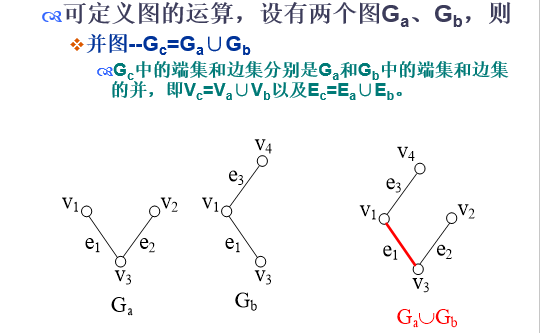
\includegraphics[width=0.5\linewidth]{figures/screenshot039}
		\caption{}
		\label{fig:screenshot039}
	\end{figure}
	\item[交图] 
	\begin{figure}[H]
		\centering
		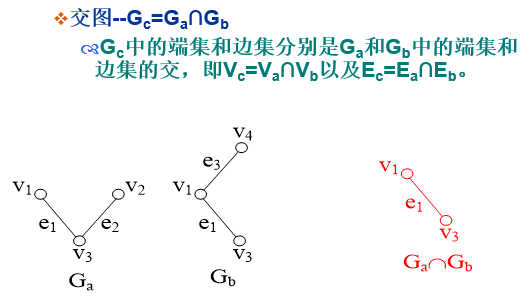
\includegraphics[width=0.7\linewidth]{figures/screenshot040}
		\caption{}
		\label{fig:screenshot040}
	\end{figure}
	\item[差图]
	 \begin{figure}[H]
		\centering
		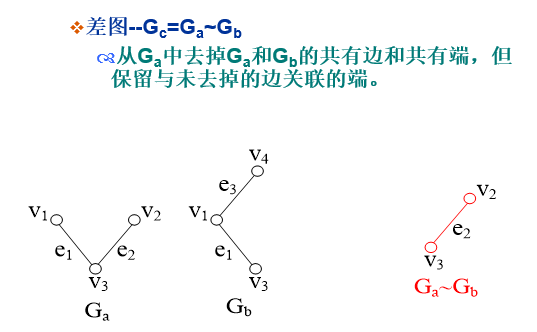
\includegraphics[width=0.7\linewidth]{figures/screenshot041}
		\caption{}
		\label{fig:screenshot041}
	\end{figure}
	一般来说:$ G_a ~ G_b = G_a - G_a\cap G_b $ ,所以该运算要分方向
	\item[环合图] 
	\begin{figure}[H]
		\centering
		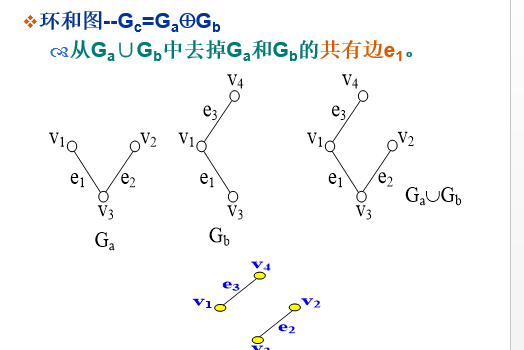
\includegraphics[width=0.7\linewidth]{figures/screenshot042}
		\caption{}
		\label{fig:screenshot042}
	\end{figure}
\end{description}
\subsubsection{图的联结性}
\begin{description}
	\item[1.端的度数] 与端相关的变数为该端的度数,自环度数+2.在有向图中$ d^+(v_i) $表示离开$ v_i $的边数,$ d^-(v_i) $表示进入,$ v_i $的度数。
\end{description}
\textbf{图的度数性质:}
对于有n个端,m条边的无向图
\begin{equation}\label{key}
\sum_{i=1}^{n}d(v_i) = 2m
\end{equation}
若G为有向图
\begin{equation}\label{key}
\sum_{i=1}^{n}d^+(v_i) = \sum_{i=1}^{n}d^-(v_i) = m
\end{equation}
任意图中,\textbf{度为奇数数的端的数目必为偶数}。
\subsubsection{链、径和还}
\begin{description}
	\item[边序列] 有限条边的一种串序排列称为边序列,要求相邻两边有公共端。(边可重复)
	\item [链] 没有重复边的链
	\item [环] 起点和终点为同一端的链
	\item[径] 无重复边、无重复端的边序列
\end{description}
\subsubsection{连接图}
\textbf{联结图的一般定义}:图内任何2个端之间至少有一条径,这图就称为联结图(或称连通图)。否则就是非联结图(或非连通图)\\
非连接图总可以分为几个部分,所谓部分是指原图的一个子图,该子图\textbf{是一个最大连接图}
\begin{figure}[H]
	\centering
	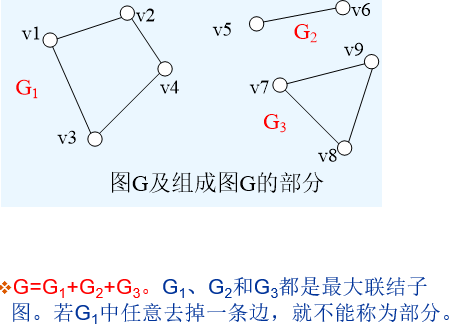
\includegraphics[width=0.7\linewidth]{screenshot003}
	\caption{}
	\label{fig:screenshot003}
\end{figure}
\subsubsection{几种特殊的连接图}
\begin{enumerate}
	\item \textbf{全连接图}:任意两端都有边的无向图成为全连接图。其边m和端n的关系
	\begin{equation}\label{key}
	m = C_n^2 = \frac{n(n-1)}{2}
	\end{equation}
	\item \textbf{两部图}:端点集合可分为2个部分,所有边的2个邻端分别在这2个集合中。特别,\textbf{完全两部图}Km,n的端点集合有2个部分,分别有m和n个端点;从2个端集合中各任取一个端,它们之间都有一条边,共有mn条边。
	\item 正则图:所有段的度数都相等
	\item 欧拉图:端度数均为偶数(不一定为连接图)。\\
连接欧拉图<=>存在一个含全边的环		
	\item M图:如果图中只有2个度数为奇数的端,则此图称为M图。
	\item 汉密尔顿(Hamilton)图:当图中至少存在一个含有所有端的环,这个图称为汉密尔顿图(也称哈密顿图),上述的环称为汉密尔顿环。
\end{enumerate}

\section{树}
定义:任何二端间有径且只有一条径的图
\subsection{基本性质}
\begin{enumerate}
	\item 树是无环的连接图
	\item 树是最小连通图。去掉任意一边就变成非连接图
	\item 若树有m条边及n个端,则有\textbf{m=n-1}
	\item 除单点树外,树\textbf{至少有2个端的度数为1}
\end{enumerate}
\subsection{主树}
生成树:包含所有端点,一定为连通图,可能不止一个
\subsection{树枝与连枝}
对于图的某一棵主树而言,主树上的边称为树枝,非树枝的边称为连枝。
主树就是树枝集;
连枝的边集称为连枝集或称为树补。
\subsection{图G的阶及其空度
}
\subsubsection{阶}
联结图G的主树T的树枝数称为图G的阶。
若图G有n个端,则它的阶$ \rho $为
$ \rho $(G)=$ \rho$=| T|=mT=n-1
\subsubsection{空度}
联结图G的连枝集的连枝数称为图G的空度,记为$ \mu $。
当G有m条边时,有\textbf{$  \mu(G)=|G-T|=m-n+ $1} 且 r+m=m
\begin{itemize}
	\item $ \mu $越大,连枝数越多,图G的联结性越好。
	\item $ \mu = 0 $表示最低联结性,即G是最小连接图。
\end{itemize}
\subsubsection{主林与林补}
对一个非联结图G,它可分成k个部分,也就是k个最大联结图。每个部分至少有一棵主树。这可找到k棵主树,所形成的集称为主林。余下的边所形成的集称为林补。
此时,G的阶可定义为主林的边数,G的空度为林补的边数。
\[ 
\rho(G)=(n1-1)+(n2-1)+….+(nk-1)=n-k
\rho+\mu=m
\mu(G)=m-n+k
\]
\section{割和环}
\subsection{割}
割是指图的某些子集,\textbf{去掉这些子集就使图的部分数增}加。若图是联结的,去掉这种子集就成为非联结图。\\
根据这种子集的元素不同,可分为割端集和割边集。
\subsubsection{割端与割端集}
\subsubsubsection{割端}
\textbf{割端:}令v是G的一个端,在去掉v和与之关联的边后,若使G的部分数增加,则称v是G的割端。
\subsubsubsection{割端集}
\textbf{割端集}:去掉几个端后,部分数增加,则这些端的集称为割端集。\\
\textbf{最小割端集中的端数},称为图的联结度,表示要破坏图的联结性的难度;联结度愈大,联结性愈不易被破坏。
\subsubsection{割边集和割集}
\textbf{割边集}:令S是联结图G的边子集,如果在G中去掉S能使G成为非联结图,则称S是G的割边集\\
\textbf{割集}:\textbf{若S的任何真子集都不是割边集},称S是割集。
实际上\textbf{,割集是最小割边集}。\\
\textbf{最小割集的边数称为图的结合度,表示图的联结程度。}
\subsection{联结度、结合度、连通度}
\begin{itemize}
	\item 联结度:最小割端集的端数称为图的联结度。
	\item 结合度:最小割集的边数称为图的结合度。
	\item 连通度:联结度和结合度统称为连通度。
\end{itemize}
\textbf{联结度是点连通度;
结合度是边连通度}
对于通信网来说,连通度越高,可靠性越好
\subsection{基本割集}
设T是联结图G的一棵主树,取一条树枝与\textbf{某些连枝}一定能构成一个割集,这种割集称为基本割集。\\
基本割集只含一条树枝\\
若G有n个端,则主树有n-1条树枝,所以有$ n-1 $个基本割集\\
基本割集有$ n-1 $,由基本割集及其\textbf{环和}共形成$ 2^(n-1)-1 $(二项式求和),然后排除重复的地方。                                \begin{figure}[H]
	\centering
	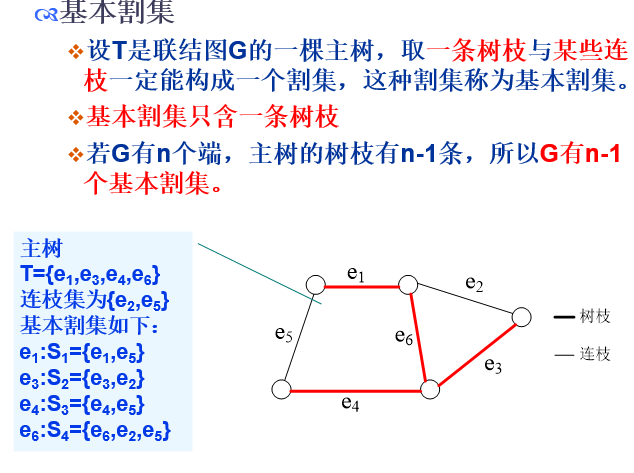
\includegraphics[width=0.7\linewidth]{figures/screenshot045}
	\caption{}
	\label{fig:screenshot045}
\end{figure}
 \subsection{基本环和所有环的方法}                              
取一条连枝可与某些树枝构成\textbf{闭径或环}。这种仅包含有一条连枝的环称为联结图的\textbf{基本环}。显然,基本环的数目等于连枝数\textbf{m-n+1}。
基本环的环和可组成$ 2^{m-n+1}-1 $个元,每个元或为环,或为环的并。
\begin{figure}[H]
	\centering
	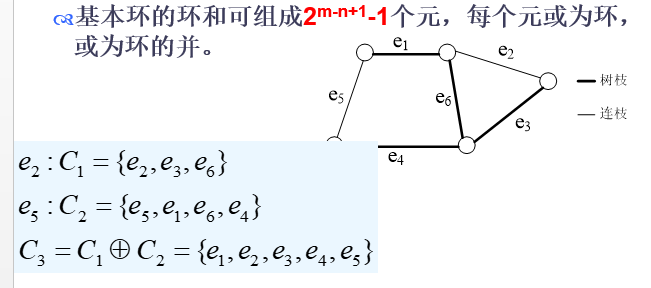
\includegraphics[width=0.7\linewidth]{figures/screenshot044}
	\caption{}
	\label{fig:screenshot044}
\end{figure}















